%!TEX root = ../memoire.tex

\chapter{GenDR}\label{chapgendr}

GenDR (Generic Deep Realizer) est un réalisateur profond multilingue \citep{lareau18}. Il a hérité de l'architecture de MARQUIS \cite{WannerMARQUISGENERATIONUSERTAILORED2010} que nous avons présenté à la section \ref{sectionmarquis}. GenDR modélise le langage dans des paramètres similaires à ceux de son prédecesseur. La réalisation linguistique se fait via la transduction de graphes, la théorie Sens-Texte est aussi le cadre utilisé, et les mécanismes permettant la transduction de graphes (dictionnaires et règles de grammaire) fonctionnent essentiellement de la même manière. GenDr a aussi repris la \ac{TST} comme théorie linguistique car c'est une théorie qui a fait ses preuves en matière de \ac{GAT} si on se fie à MARQUIS \citep{WannerMARQUISGENERATIONUSERTAILORED2010}, FORGe \citep{MilledemoFORGePompeu2017}, RealPro \citep{LavoieFastPortableRealizer1997} qui l'utilisent. De plus, \cite{Vicentegeneracionlenguajenatural2015} dans un article concernant l'état de l'art en \ac{GAT} mentionne ce cadre théorique comme étant une bonne interface pour modéliser le langage.

GenDR se démarque par sa capacité à traiter des phénomènes langagiers complexes: les collocations. Il offre une couverture beaucoup plus importante que MARQUIS en ce qui concerne les collocations via un traitement exhaustif des fonctions lexicales. Cette couverture lexicale a été opérée par Lareau et Lambrey \cite{LambreyImplementationcollocationspour2017}, \cite{lambrey15} en travaillant sur un générateur de collocations. Toutefois, il est important de préciser que GenDR réalise en sortie des structures syntaxiques de surface. Le réalisateur se concentre principalement sur l'interface sémantique-syntaxe car c'est là qu'on peut modéliser des phénomènes langagiers profonds. Pour compléter la réalisation jusqu'à du texte, il faudrait utiliser un réalisateur de surface qui prendrait les outputs de GenDR.

En tant qu'héritier de MARQUIS, GenDR a repris les modules grammaticaux de base de son prédecesseur. Les auteurs de GenDR ont gardé les règles de base décrivant des phénomènes langagiers élémentaires comme la  lexicalisation simple, la complémentation, la modification (adjectivale et adverbiale),etc. Ces règles forment le noyau du système et sont généralement partagées par l'ensemble des langues. Puis, des phénomènes comme la sélection des auxilaires ou des déterminants sont régis par des règles spécifiques à chaque langue

\draft{ où est-ce que j'incorpore ça dans mon texte: Le module sémantique contient 21 règles dont la plupart sont héritées de MARQUIS et 132 règles de lexicalisation \citep{LambreyImplementationcollocationspour2017}. Le module syntaxique contient nettement moins de règles. 20 règles dont 12 partagées entre les langues. }

%%%%%%%%%%%%%%%%%%%%%%%%%%%%%%%%%%%%%%%%%%%%%%%%%%%%%%%
% --------- A R C H I T E C T U R E  GENDR  ---
%%%%%%%%%%%%%%%%%%%%%%%%%%%%%%%%%%%%%%%%%%%%%%%%%%%%%%%
\section{Architecture de GenDR}

Les modules lexicaux et grammaticaux de GenDR sont pris en charge par un transducteur de graphes du nom de MATE \citep{BohnetDevelopmentEnvironmentMTTbased2000}. Donc pour mieux comprendre comme la réalisation se déroule dans GenDR, il faut d'abord présenté comment fonctionne MATE et quels sont les modules utilisés dans MATE pour générer du texte.

\subsection{MATE}
MATE a été créé par \cite{BohnetDevelopmentEnvironmentMTTbased2000} pour implémenter un système se basant sur la Théorie Sens-Texte. Dans ce contexte, chaque niveau de représentation est traduit par un graphe. Le transfert de ceux-ci est assuré par un module de dictionnaire et de grammaire. La réalisation de texte se fait donc grâce aux transductions de graphes. Effectivement, MARQUIS utilisait ce système de transduction de graphes pour réaliser le texte final \citep{Lareau2007TowardsAG}. MATE a aussi été conçu pour tester, développer et maintenir une grammaire computationnelle. C'est un logiciel qui permet à la fois de réaliser du texte et de tester des fondements théoriques dans une application concrète. 

Pour réaliser du texte, MATE comprend les composantes suivantes : un éditeur de dictionnaires, de graphes et de grammaires. Les dictionnaires encodent les unités sémantiques et lexicales. Les grammaires sont composées de règles modélisant le passage d'une représentation à une autre. L'éditeur de graphes permet de construire l'input et de le visualiser soit en format textuel ou graphique. Il y aussi un module d'inspecteur permettant de voir le déroulement de l'application des règles. Cet outil s'avère très utile au développement d'une grammaire. On peut cerner à quel endroit la réalisation s'est interrompue et à cause de quel module. Pour plus de détails concernant ce système, nous vous référons à ces articles: \citep{BohnetOpensourcegraph2010} et \citep{LambreyImplementationcollocationspour2017}.

Nous allons maintenant montrer brièvement à quoi ressemble les éditeurs dictionnairiques, grammaticaux et graphiques.
%%%%%%%%%%%%%%%%%%%%%%%%%%%%%%%%%%%%%%%%%%%%%%%%%%%%%%%
% ---------D I C T I O N N A I R E  ------------------
%%%%%%%%%%%%%%%%%%%%%%%%%%%%%%%%%%%%%%%%%%%%%%%%%%%%%%%

\subsubsection{Dictionnaires}\label{dictio}

Tel que nous l'avons mentionné, GenDR se sert de dictionnaire pour encoder le lexique qui sera utilisé dans les réalisations finales. Le système se sert de trois dictionnaires: un dictionnaire sémantique, un dictionnaire lexical et un dictionnaire de fonctions lexicales. Puisque les fonctions lexicales en génération automatique de texte ont déjà traitées par \cite{LambreyImplementationcollocationspour2017}, nous ne traiterons pas de ce dictionnaire ici. 

Nous commencerons par décrire le dictionnaire sémantique car c'est le premier dictionnaire qui est requisitionné par le système lors du passage de la représentation sémantique à la représentation syntaxique profonde. Il sert à encoder les unités sémantiques se trouvant dans les graphes d'entrées. La figure \ref{semanticon} présente une entrée typique dans un dictionnaire sémantique (\emph{semanticon}).

\begin{lstlisting}[language=Xml, caption=Semanticon, label=semanticon]
owe { lex = owe
      lex = debt }
\end{lstlisting}

Le \emph{semanticon} mappe les sémantèmes à des lexèmes ou des locutions. Ce dictionnaire est à la base de nombreuses réalisation de paraphrases. La raison est simple, une unité sémantique peut se réaliser de plus d'une manière en fonction de la synonymie ou du changement de partie du discours. C'est pour cela que, dans la figure \ref{semanticon}, le sens de \sem{owe} englobe deux réalisations lexicales: \lex{owe} et \lex{debt}. La première est un lexème verbal et la seconde est un lexème nominal.

\draft{comment mettre les {} dans lstline ?}Passons ensuite au dictionnaire lexical \emph{lexicon}. Il contient de l'information détaillée à propos de chaque unité lexicale d'une langue donnée. Une entrée lexicale typique contient: la partie du discours, la diathèse, les patrons de régime, et les collocations contrôlées. D'ailleurs, comme vous le verrez dans la figure \ref{lexicon}, ces informations lexicales ne sont pas toujours explicitée, mais elles sont quand même encodées dans l'entrée. Cela est possible via un mécanisme d'héritage propre à MATE. Autrement dit, le verbe \lex{owe} ne semble que contenir les patrons de régime dans son entrée lexicale. Toutefois, grâce au mécanisme d'héritage récursif, il hérite d'une panoplie de traits. Vous verrez que cette entrée lexicale pointe vers \emph{verb\_dit} (verbe ditransitif). C'est là que le mécanisme d'héritage des traits entre en jeu. \lex{Owe} hérite de toutes les informations encodées dans \emph{verb\_dit}. Notamment son patron de régime. Puis sucessivement, la classe \emph{verb\_dit} hérite des traits de \emph{verb\_dt} puis de \emph{verb} et finalement de \emph{predicate}. Ce système a donc permi à \lex{owe} d'hériter de tous les traits encodés dans ces classes: la diathèse via \lstinline!gp = { 1 = I ,...} !, la partie du discours \lstinline{dpos = V} et les patrons de régime \lstinline!gp = { III = { dpos = N rel = indir\_objective prep = to }! retrouvés dans chaque classe. Cela permet à MATE de ne pas être saturé d'information et facilite l'encodage des unités lexicales. Les concepts de classes ne se limitent pas qu'aux différents type de verbes (transitif, intransitif,etc.) mais aussi aux partie du discours: les adjectifs, les adverbes, les noms, les prépositions, etc. C'est de cette manière que le lexicon fonctionne. On spécifie les traits lexicaux dans des classes, puis on associe les entrées lexicales à ces classes pour qu'elles héritent des traits. Si c'est nécessaire qu'un des traits soit modifié, on peut le faire directement dans l'entrée lexicale. La lexie \lex{owe} en montre un exemple en modifiant la partie du discours (Num) demandée par son deuxième actant syntaxique \lstinline!gp = { II = { dpos=Num } }!. Nous avions mentionné le pouvoir de paraphrasage dans le chapitre précédent. Le lexème \lex{debt} contient les collocations qu'il contrôle. La réalisation de ces collocations se fait par l'entremise d'un dictionnaire de fonction lexicale puisque \lex{debt} nécessitera un verbe support pour pouvoir paraphraser le sens de \sem{owe}. Pour plus de détails nous vous renvoyons à \citep{lareau18} et \citep{LambreyImplementationcollocationspour2017}.

\begin{lstlisting}[language=Xml, caption = Lexicon, label=lexicon]
predicate {
  gp = { 1 = I
         2 = II
         3 = III
         4 = IV
         5 = V
         6 = VI }
}

verb : predicate {
  dpos = V
  spos = verb
  gp = {
     I = {
        dpos = N
        rel = subjective
     }
  }
}

verb_dt : verb {                   // direct transitive
  gp = {
     II = {
        dpos = N
        rel = dir_objective

     }
  }
}

verb_dit : verb_dt {                   // direct ditransitive
  gp = {
     III = {
        dpos = N
        rel = indir_objective
        prep = to  

     }
  }
}
[...]
owe : verb_dit {
  gp = { II = { dpos=Num } }
  gp = { II = { dpos=N } }
}

debt : noun {
  gp = {
    1 = II
    2 = I
    3 = III
    I = { dpos=Num rel=noun_completive prep=of }
    II = { dpos=N rel=determinative case=GEN prep=""}
    III = { dpos=N rel=noun_completive prep=to }
  }
  lf = { name=Oper1 value=have }
  lf = { name=Oper13 value=owe }
  lf = { name=Func2 value=amount_v_1 }
  lf = { name=Func2 value=stand_v_2 }
  lf = { name=Func2 value=total_v }
}
\end{lstlisting}

Finalement, pour conclure la section sur les dictionnaires, nous mentionnerons quelques statistiques. Le dictionnaire anglais de GenDR contient les 1500 lexèmes les plus courants. Le dictionnaire francophone en contient autant. Puis les dictionnaires lithuanien et persan contiennent quelques lexèmes afin de pouvoir tester le système et réaliser quelques phrases.

%%%%%%%%%%%%%%%%%%%%%%%%%%%%%%%%%%%%%%%%%%%%%%%%%%%%%%%
% ---------G R A M M A I R E  ------------------
%%%%%%%%%%%%%%%%%%%%%%%%%%%%%%%%%%%%%%%%%%%%%%%%%%%%%%%

\subsubsection{Grammaires}

La grammaire de GenDR est organisée autour de deux modules englobant des règles. Le premier module est celui qui permet le passage de la sémantique (input) à la syntaxe profonde (intermédiaire). Puis le second module permet le passage de la syntaxe profonde à la syntaxe de surface (output). Le premier module est divisé en 3 sections: les règles partagées par tous (\emph{core}), les règles de fonctions lexicales (\emph{lf}), et les règles spécifiques à chaque langue (\emph{lng}).	Le second module est divisé en 2: les règles partagées par tous et les règles propres à chaque langues. Nous présenterons en détails les règles principales de ces deux modules dans les sections \ref{secarbolex} et \ref{secexemple}. \draft{élaborer sur les différentes sections du core: syntax, lexical, root ?}

La figure \ref{fig:root} présente une règle du module sémantique-syntaxe profonde. Toutes les règles sont décrites dans ce format. D'abord, en haut, on a l'interface dans laquelle la règle opère et le nom de la règle. Dans la partie gauche \emph{Leftside} on retrouve les noeuds et arcs du graphes de départ, puis dans la partie droite \emph{Rightside} on retrouve le graphe de sortie avec les noeuds et arcs qui ont subi des transformations. Finalement, la partie d'en bas concerne les conditions d'applications. Il s'agit d'un ensemble de conditions restreignant le champ d'application de la règle donnée. Nous verrons en détails l'application concrète de la règle \ref{fig:root} dans la section \ref{secarbolex}.
\begin{figure}[htb]
	\centering
	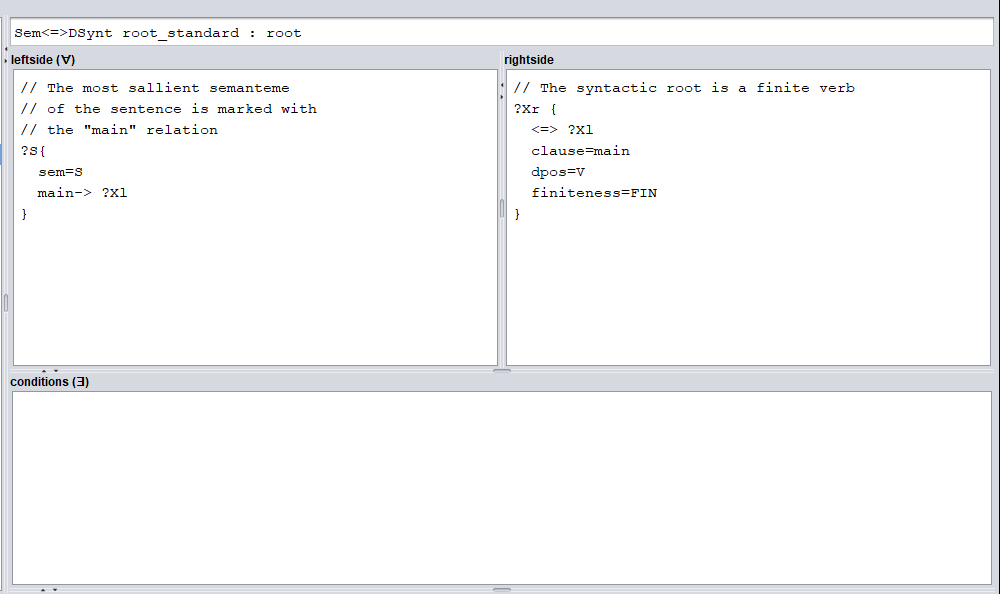
\includegraphics[width=1\textwidth, trim = {0cm 0cm 0cm 0cm},clip]{ch3/figs/grammaire.png}
	\caption{Règle créant la racine syntaxique}
	\label{fig:root}
\end{figure}

%%%%%%%%%%%%%%%%%%%%%%%%%%%%%%%%%%%%%%%%%%%%%%%%
% ---------G R A P H E S ------------------
%%%%%%%%%%%%%%%%%%%%%%%%%%%%%%%%%%%%%%%%%%%%%%%%

\subsubsection{Graphes}\label{entree-sortie}
Maitenant que nous avons fait un survol des dictionnaires et des modules de grammaires, il ne nous reste qu'à présenter les graphes. Dans un premier temps nous présenterons brièvement à quoi ressemble la construction d'un graphe en input. Puis nous montrerons à quoi ressemble les graphes en output.

L'input du réalisateur GenDR est un graphe sémantique de type \acf{TST}. Dans celui-ci les prédicats sont liés à leurs arguments par des relations étiquettées avec des chiffres qui indiquent la position de l'argument. La figure \ref{input} montre comment on construit un graphe sémantique dans MATE.

\begin{lstlisting}[language=XML, caption = Input sémantique, label=input]
structure Sem debt {
S {
owe {
tense=PRES
1-> Paul {class=proper_noun}
2-> "\$500K" {class=amount}
3-> bank {number=SG definiteness=DEF}}
main-> owe}}
\end{lstlisting}

Toutefois, MATE offre aussi une version graphique pour encoder et visualiser le graphe sémantique (voir la figure \ref{fig:graphesem}).
\begin{figure}[htb]
	\centering
	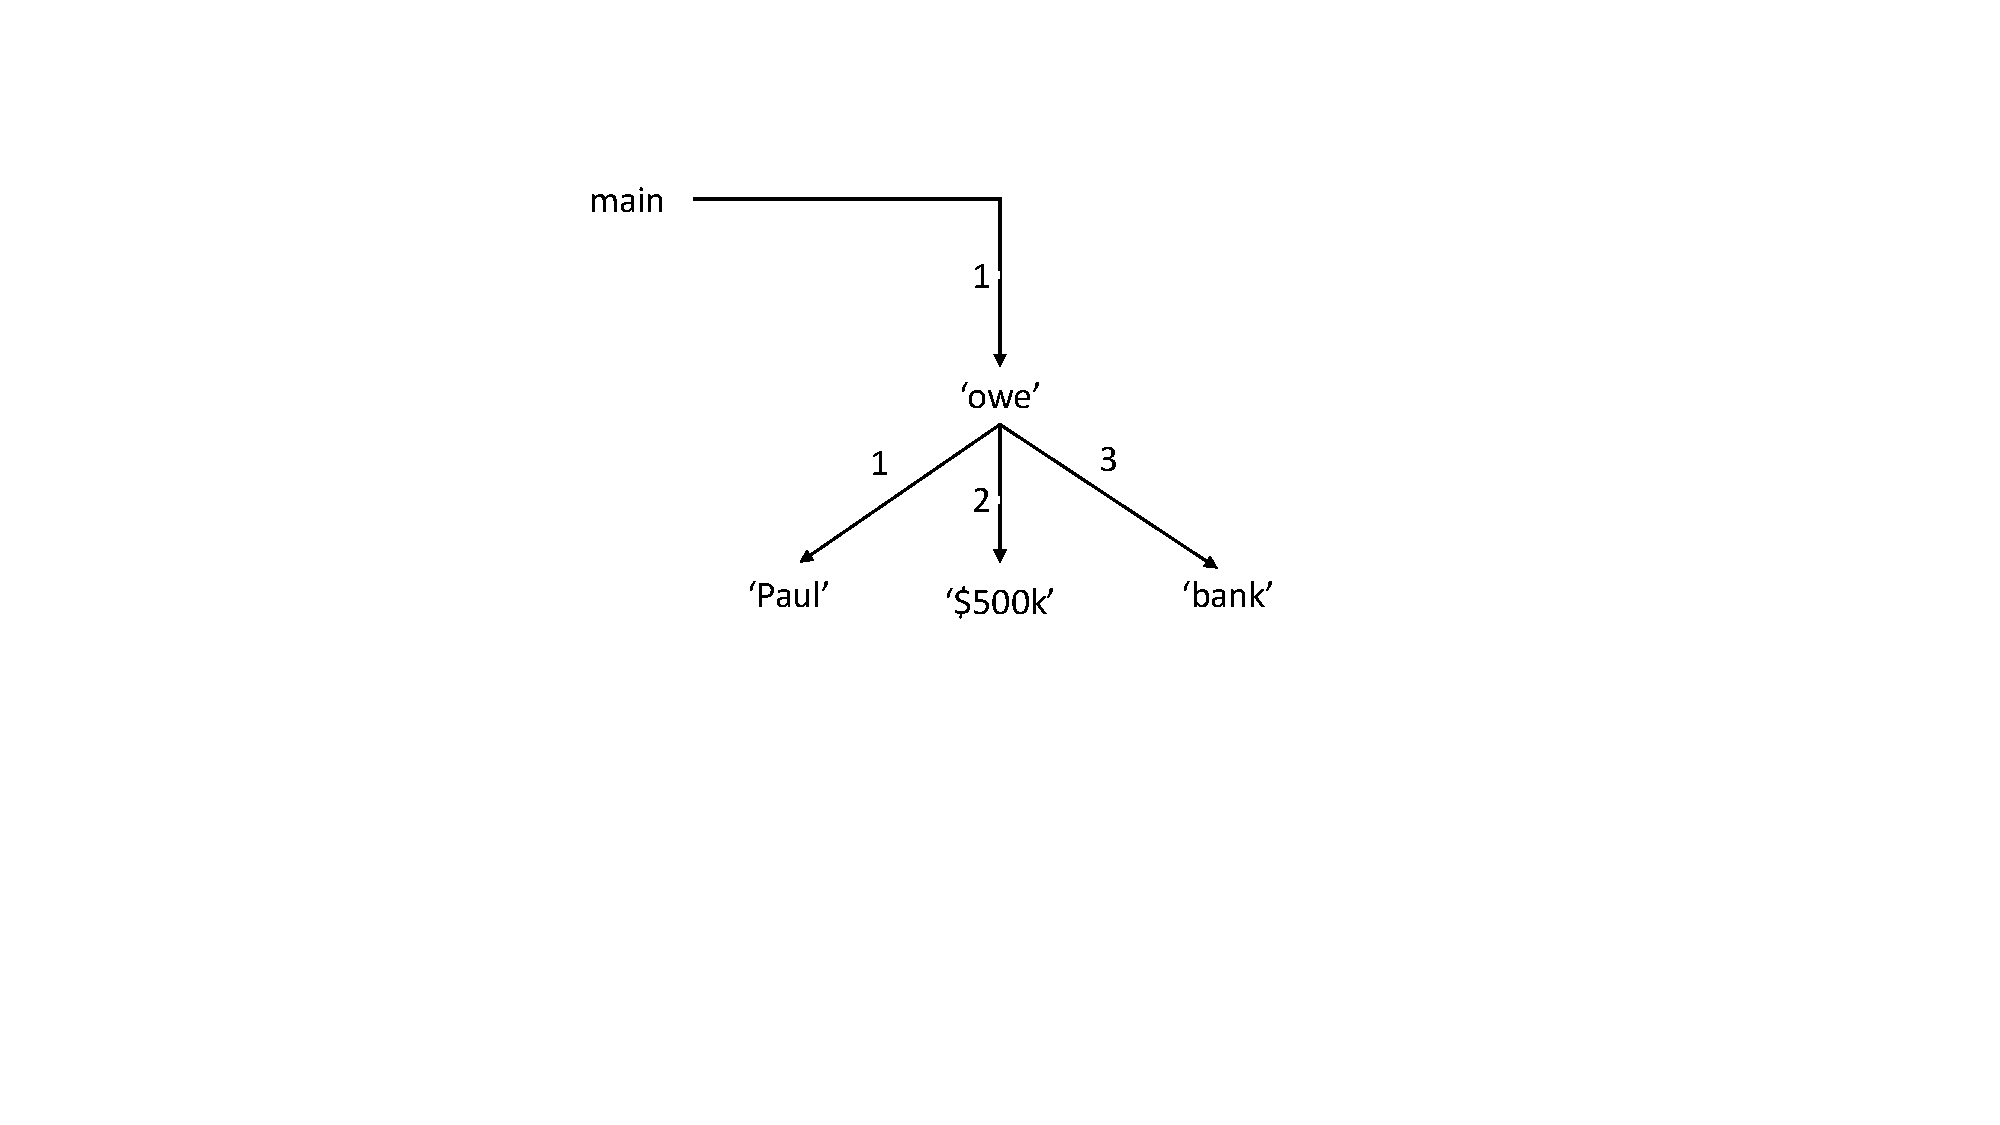
\includegraphics[width=1\textwidth, trim = {0cm 4cm 0cm 3cm},clip]{ch3/figs/owe_sem.pdf}
	\caption{Graphe sémantique en visuel}
	\label{fig:graphesem}
\end{figure}

La section graphe de GenDR nous permet de construire les structures sémantiques d'input et de visualiser les transductions de graphes. Pour l'input donné en \ref{input}, GenDR réalise six structures syntaxiques de surface. Celles-ci peuvent être visualisées dans MATE grâce au module de graphes. La figure \ref{fig:realsurfex} est un exemple d'output visuel que fournirait MATE. 

\begin{figure}[htb]
	\centering
	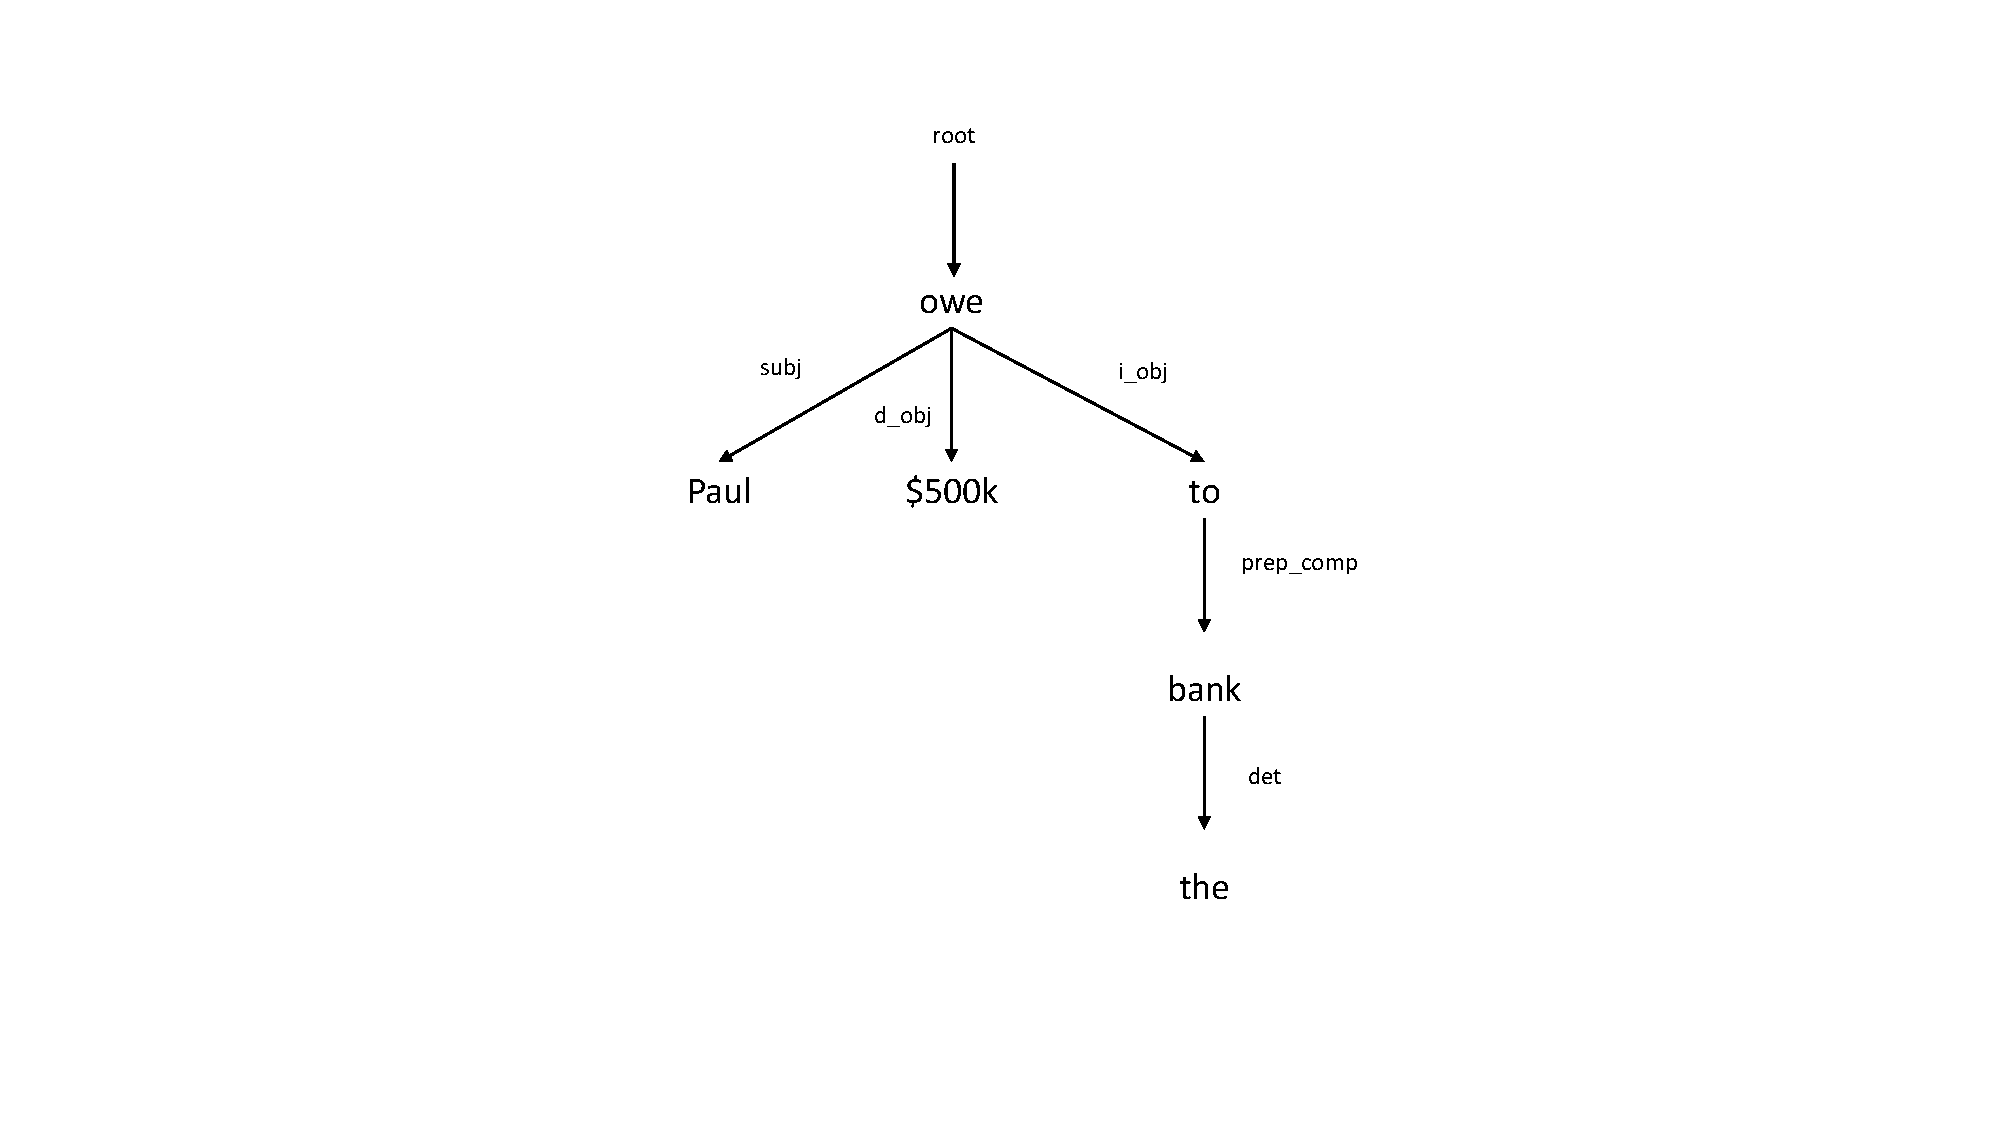
\includegraphics[width=1\textwidth, trim = {0cm 2cm 0cm 2cm},clip]{ch3/figs/realsurfex.pdf}
	\caption{Réalisation de surface}
	\label{fig:realsurfex}
\end{figure}

Toutefois, les modules de règles et de dictionnaires permettent en réalité de réaliser de six arbres syntaxiques superficiels (grâce aux mécanismes de paraphrasage). Nous les présentons à la figure \ref{fig:6realsurf}. Dans cette figure, les arbres de dépendances ont été linéarisés pour faciliter la compréhension du lecteur. Dans les faits, les arbres générés en output ne sont pas linéarisés et ils ressemblent à ceux de la figure \ref{fig:realsurfex}.

\begin{figure}[htb]
	\centering
	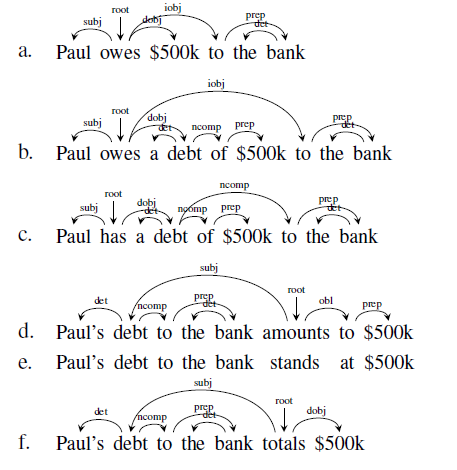
\includegraphics[width=0.5\textwidth, trim = {0cm 0cm 0cm 0cm},clip]{ch3/figs/exemples_real.png}
	\caption{6 réalisations syntaxe de surface}
	\label{fig:6realsurf}
\end{figure}

Si on souhaite une réalisation linéarisée,  il faudra utiliser un réalisateur de surface. GenDR ne traite pas l'interface morpho-syntaxique et ne linéarise pas le texte. C'est exactement dans ces contextes, que les réalisateurs de surface comme SimpleNLG ou JSreal \cite{DaoustJSREALTextRealizer2015}\cite{MolinsJSrealBBilingualText2015}\cite{GattSimpleNLGRealisationEngine2009}entrent en jeu. Au lieu de mettre des efforts à réaliser le texte jusqu'à la fin, GenDR a concentré ses efforts à effectuer des tâches plus abstraites modélisant des phénomènes langagiers complexes. L'arborisation et la lexicalisation sont principalement les deux tâches où GenDR s'est démarqué des autres réalisateurs profonds. Nous les expliquerons en détails dans la section \ref{secsemsynt}.

%%%%%%%%%%%%%%%%%%%%%%%%%%%%%%%%%%%%%%%%%%%%%%%%%%%%%%%%%%%%%%%%%%%%%%%%%%%%%
% --------- I N T E R F A C E   S É M A N T I Q U E- S Y N T A X E ---------
%%%%%%%%%%%%%%%%%%%%%%%%%%%%%%%%%%%%%%%%%%%%%%%%%%%%%%%%%%%%%%%%%%%%%%%%%%%%%

\section{Interface sémantique-syntaxe en TST}\label{secsemsynt}

La capacité de GenDR à réaliser plusieurs phénomèns langagiers découle du travail qui a été fait pour développer son interface sémantique-syntaxe. Dans la section présente, nous décrirons cette interface dans les termes de la \ac{TST}. Plus précisément, nous décrirons deux processus nécessaires au passage de la sémantique à la syntaxe: l'arborisation et la lexicalisation.Pour mieux comprendre ce que sont ces procédés, nous ferons un très bref retour sur la \ac{TST}. 

La \ac{TST} est une théorie qui vise la description de la correspondance entre le \emph{Sens} et le \emph{Texte}. Cette correspondance est effectuée par la construction de modèles formels \citep{PolgueretheorieSensTexte1998}. La figure \ref{fig:modeletst} provient de \citep{PolgueretheorieSensTexte1998} et elle présente comment fonctionnent ces modèles. Elle illustre le fait qu'un modèle Sens-Texte est une machine virtuelle qui prend en entrée des représentations sémantiques d'énoncés et génère un ensemble de Textes qui contiennent toutes les paraphrases permettant d'exprimer le \emph{Sens} donné en entrée. 
\begin{figure}[htb]
	\centering
	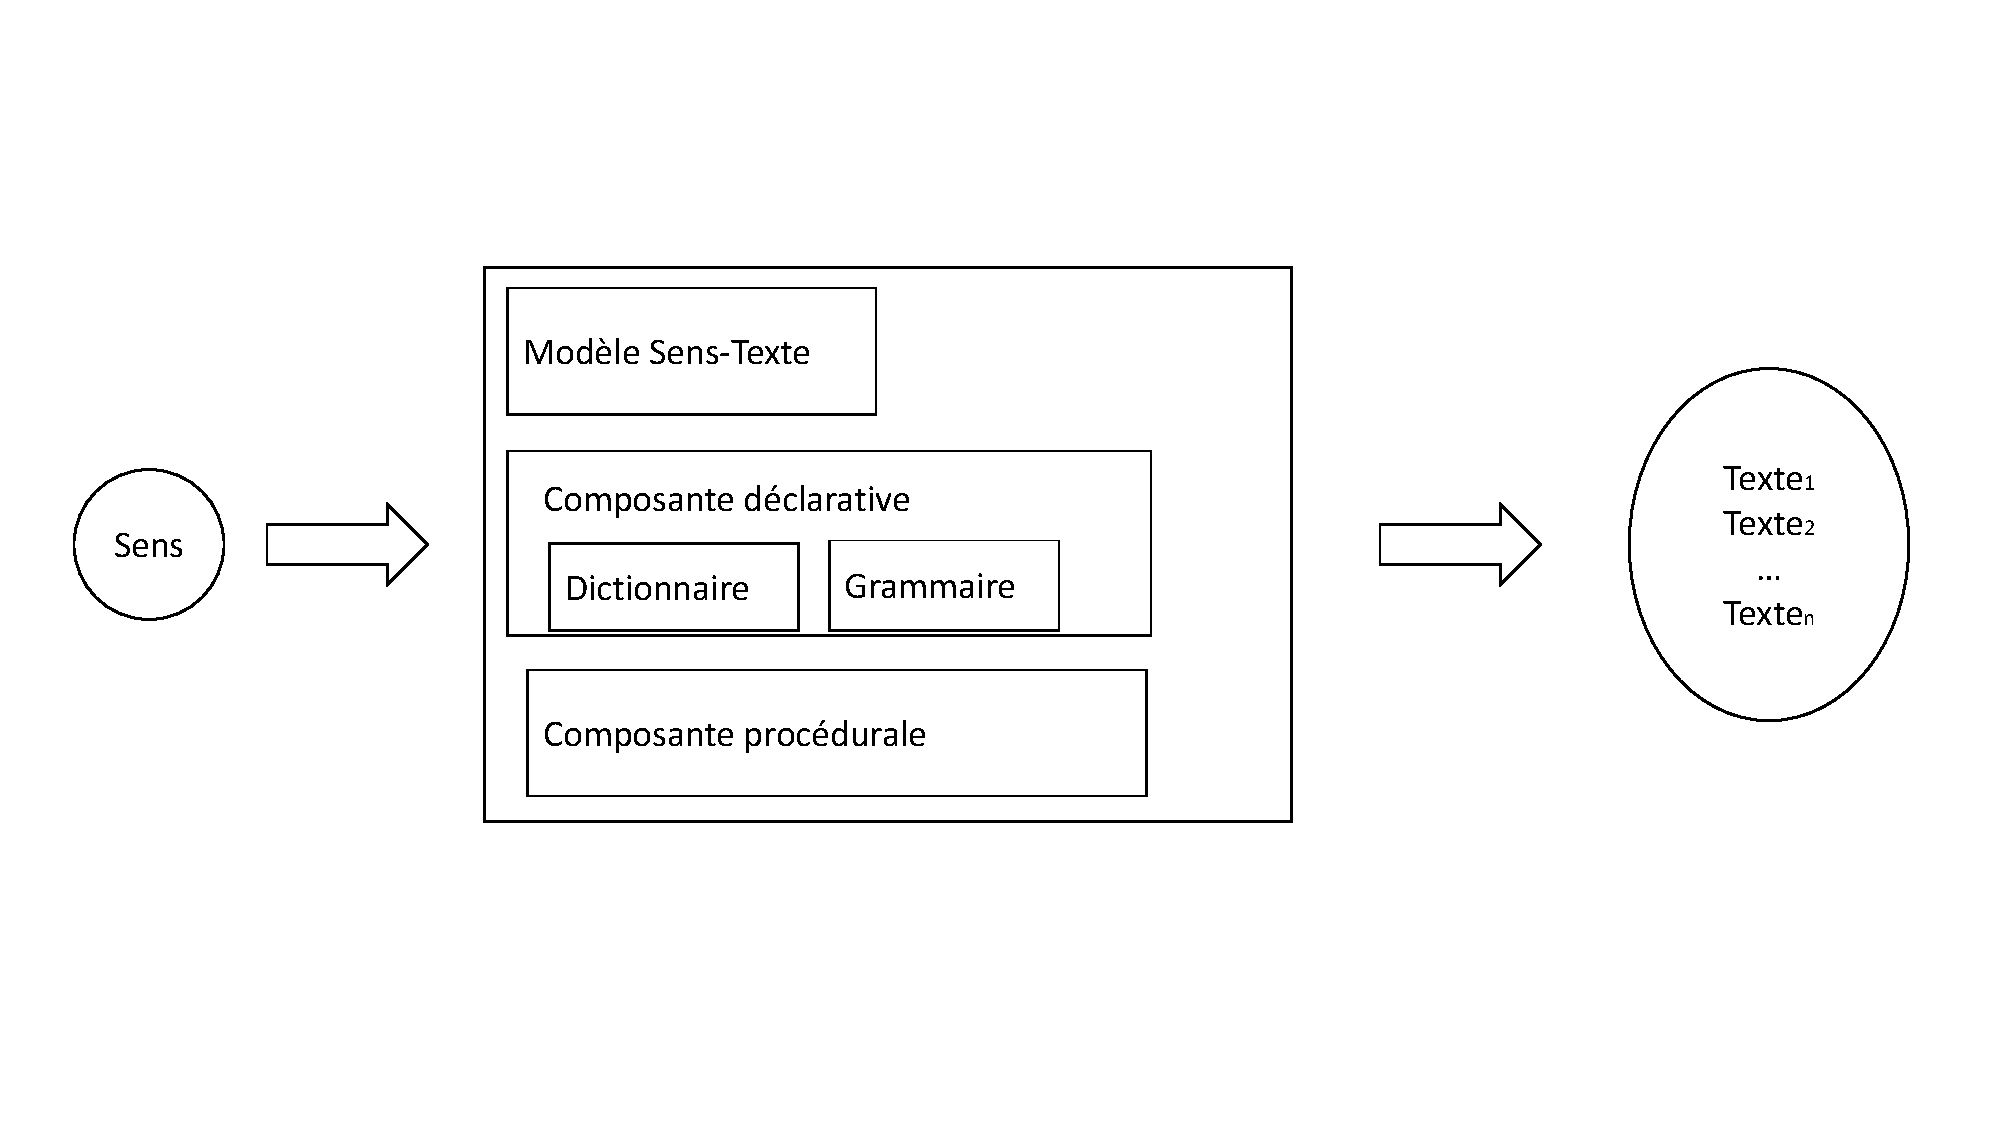
\includegraphics[width=1\textwidth, trim = {0cm 3cm 0cm 3cm},clip]{ch3/figs/polguere1.pdf}
	\caption{Structure d'un modèle TST}
	\label{fig:modeletst}
\end{figure}

Concrètement, la figure \ref{fig:modeletst} démontre comment on passe de la figure 2.4 (qui représente le \emph{Sens}) à la figure 2.6 (qui représente le \emph{Texte}). Pour se rendre au texte final, le \emph{Sens} traverse de nombreux niveaux de représentations. La figure \ref{fig:processustst} démontre les niveaux de représentations que l'input doit traverser succesivement, puis en parallèle comment on représente ces représentations au cours de la réalisation.
\begin{figure}[htb]
	\centering
	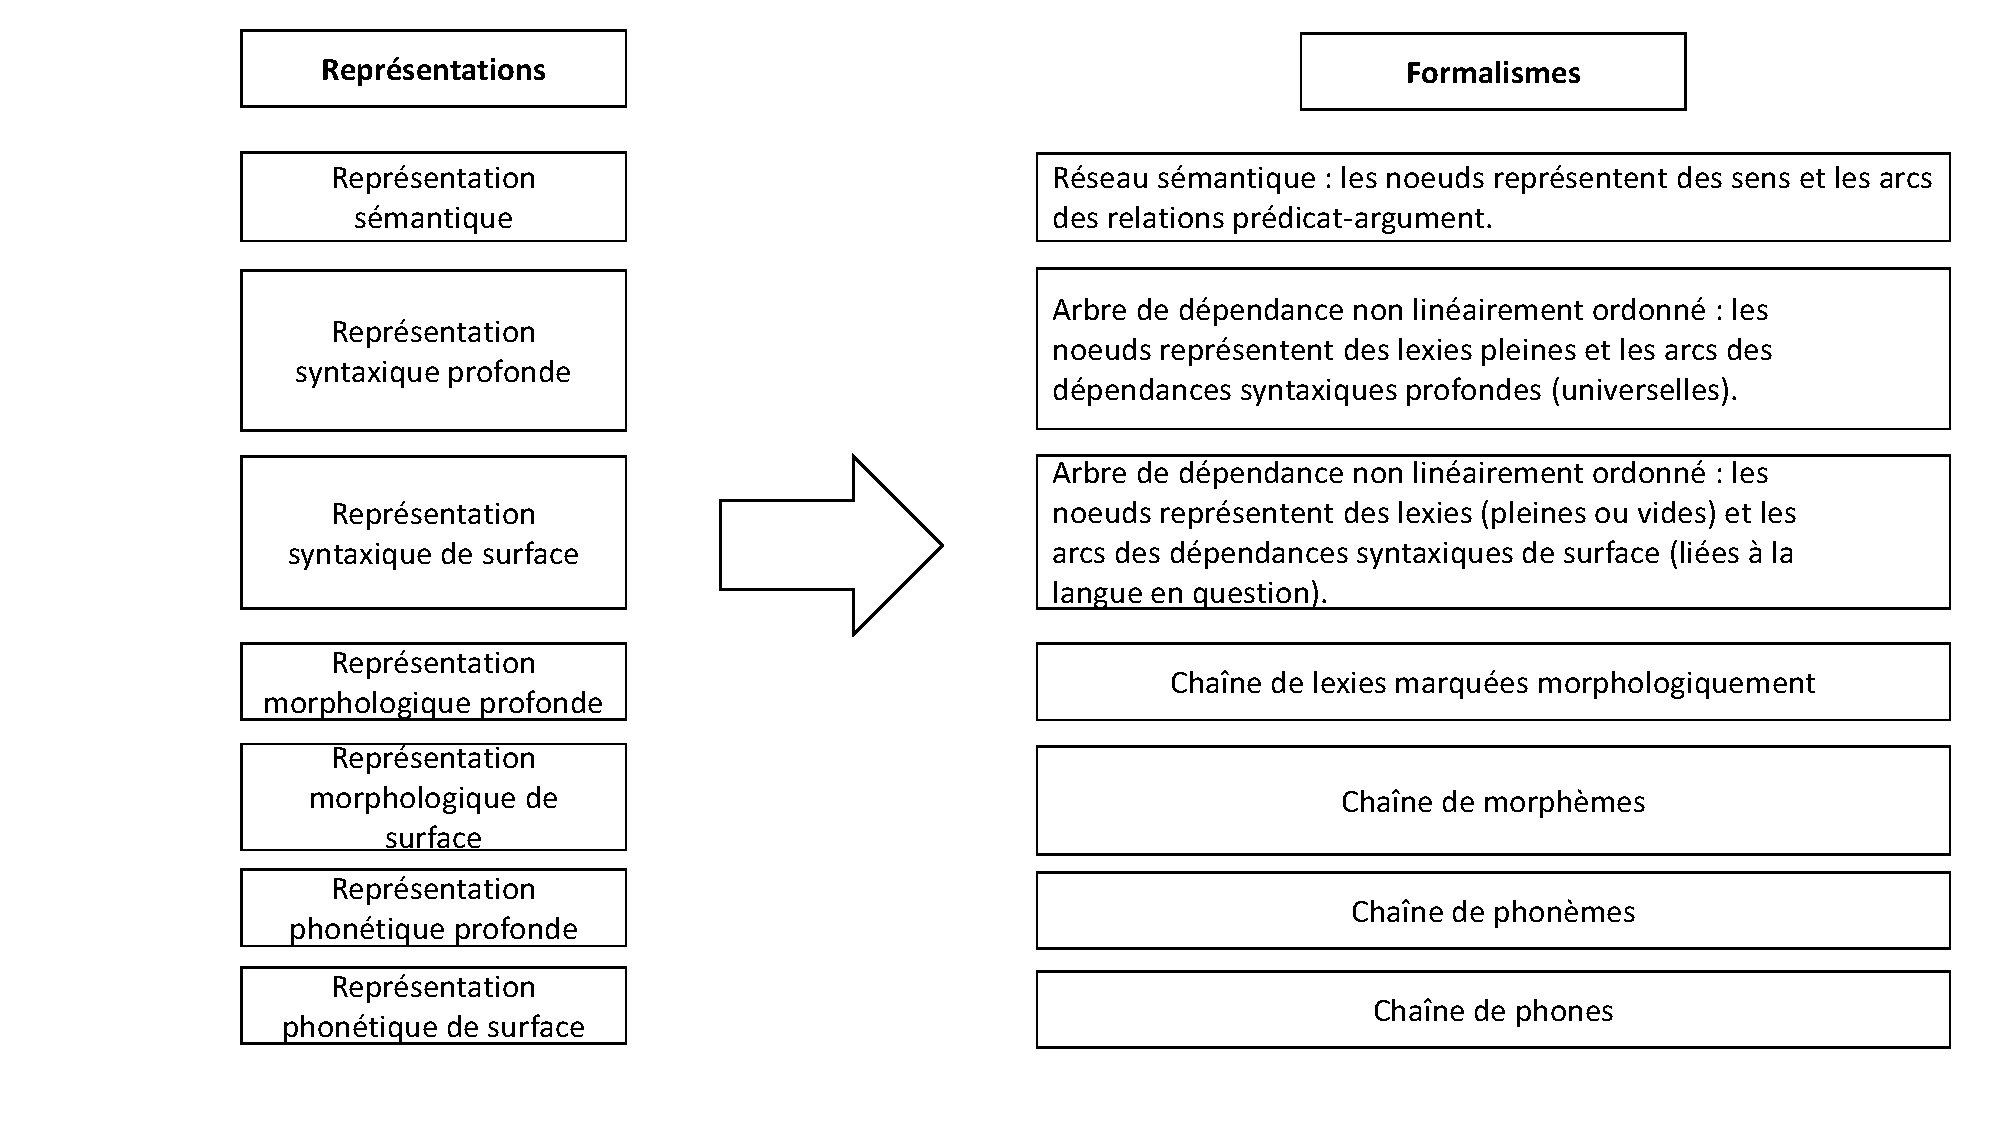
\includegraphics[width=1\textwidth, trim = {0cm 0cm 0cm 0cm},clip]{ch3/figs/polguere2.pdf}
	\caption{Processus d'un modèle TST}
	\label{fig:processustst}
\end{figure}

%%%%%%%%%%%%%%%%%%%%%%%%%%%%%%%%%%%%%%%%%%%%
% ---------T H É O R I Q U E  ------
%%%%%%%%%%%%%%%%%%%%%%%%%%%%%%%%%%%%%%%%%%%

\subsection{Arborisation théorique}\label{arbo}

Comme GenDR traverse trois niveaux de représentations, nous expliquerons uniquement les processus nécessaires à la compréhension du système. Nous commencerons par l'arborisation qui est le passage de la représentation sémantique à la représentation syntaxique profonde.

Selon la \ac{TST}, la structure syntaxique d'un énoncé représente l'ensemble des liens de dependances fonctionnelles qui existent entre les unités lexicales de cet énoncé. On représente formellement ces structures syntaxiques par des arbres qu'on appelle des arbres de dépendances. Cette approche syntaxique provient de \cite{TesniereElementssyntaxestructurale1965} qui est le premier à l'avoir théorisée.

Formellement, le passage de la RSem à la RSyntP se nomme l'arborisation. Elle est ainsi nommée  parce qu'on chercher à arboriser la RSem pour qu'il en résulte un arbre de dépendance profond. Ce passage est effectuée via des règles de correspondance sémantiques. Celles-ci forment une partie de la grammaire dans le schéma montré plutôt à la figure \ref{fig:modeletst}.

Pour que l'arborisation se fasse correctement, il faut que la racine de l'arbre en construction corresponde à un noeud sémantique identifié comme étant le plus saillant. La détermination de la racine correspond au processus de hiérarchisation \citep{PolguereStructurationmisejeu1990}. On l'appelle ainsi car la racine est le noeud qui domine tous les autres noeuds de l'arbre syntaxique profond. Une fois que c'est fait, on va trouver le lexème qui peut satisfaire les contraintes du noeud de la racine. Il faut que le lexème sélectionné corresponde à l'unité sémantique identifiée comme la plus saillante. Le lexème doit aussi satisfaire des contraintes comme la partie du discours ou la finitude. Généralement on a ces contraintes sur la racine puisque ce sont généralement les verbes qui contrôlent les énoncés. En lexicalisant le noeud, on va simultanément ajouté les arcs qui en dépendent. Ceux-ci correspondent aux arguments liés à ce prédicat dans la RSem. Comme Polguère le dit: "chaque arc est considéré successivement dans l'ordre du parcours, puis est traduit en une micro-structure syntaxique profonde grâce aux règles de correspondance sémantique de la grammaire." p.273 de \citep{PolguereStructurationmisejeu1990}. 

Une fois que l'arborisation est complétée, l'arbre de dépendance profond transitera vers le niveau de syntaxe de surface. Cette transition implique les opérations suivantes. D'abord, faire le calcul des relations syntaxiques de surface. Ainsi, la relation I deviendra sujet, la relation II deviendra complément d'objet direct, etc. De plus, on incorpore les lexies vides (prépositions, déterminants, etc.) à ce stade et on opère la pronominalisation. 

\subsection{Lexicalisation théorique}

Tel que nous l'avions présenté dans la figure \draft{figure dans MARQUIS}, la lexicalisation se produit entre la RSem et la RSyntP \citep{PolguereStructurationmisejeu1990}. Concrètement, il s'agit de la correspondance entre une unité sémantique et les lexies qu'elle contrôle. La correspondance est inscrite dans le dictionnaire sémantique et lexical. La lexicalisation est ainsi très liée à l'arborisation car ce sont deux étapes qui se produisent lors du passage de la RSem à la RSyntP. D'ailleurs, ces deux étapes se produisent successivement l'une à la suite de l'autre. La construction de la représentation syntaxique profonde est une conséquence de l'arborisation des arcs de la RSem et de la lexicalisation des unités sémantiques de cette RSem. Le tout résulte en un arbre de dépendance lexicalisé. Comme nous l'avions vu dans la figure \draft{au début}, le passage de \sem{owe} à \lex{owe} et \lex{debt} représente la lexicalisation.

%%%%%%%%%%%%%%%%%%%%%%%%%%%%%%%%%%%%%%%%%%%%%%%%%%%%%
% --------- C O M P U T A T I O N N E L L E  ------
%%%%%%%%%%%%%%%%%%%%%%%%%%%%%%%%%%%%%%%%%%%%%%%%%%%%

\section{Arborisation et lexicalisation computationnelle}\label{secarbolex}

Maintenant que nous avons présenté le côté théorique de l'interface sémantique-syntaxe, nous exposerons comment ces mécanismes se traduisent d'un point de vue computationnel dans GenDR.

\subsection{Arborisation computationnelle}
La première étape du processus d'arborisation dans GenDR est la même que celle que nous avions expliquée d'un point de vue théorique. Il faut créer la racine de l'arbre qui correspond au noeud le plus saillant de la RSem. Pour faire cela, nous devons indiquer le noeud le plus saillant dans la structure d'input (voir figure x). L'arbre syntaxique profond est construit avec un algorithme top-down qui ressemble beaucoup à celui qu'utilisent MARQUIS et FORGe puisqu'ils sont aussi des tenants de la TST. 

\subsubsection{Règles de base pour l'arborisation}
L'arborisation dans GenDR se fait en trois étapes.

Première étape. La première règle appliquée est: root\_standard. Elle construit la racine de l'arbre syntaxique à partir du noeud principal de la structure sémantique. À cette étape, la racine n'est pas étiquettée par un lexème encore (noeud vide), mais on lui impose des contraintes. La contrainte principale est qu'il doit s'agir d'un verbe à l'indicatif. Cette règle ne s'applique donc qu'une seule fois par réalisation.

Deuxième étape. Une fois que la racine a été créée et contrainte en syntaxe profonde, on applique une règle de lexicalisation. Cela permet au système de fouiller dans les dictionnaires pour un lexème qui correspondra au sens demandé et aux contraintes imposées.

Troisième étape. Une fois que le noeud racine est lexicalisé, GenDR regarde dans le patron de régime de la racine pour savoir comment faire le passage des arcs sémantiques aux arcs syntaxiques. Ceux qui partent du noeud sémantique vers ses arguments seront réalisés comme des actants syntaxiques. Tandis que les arcs qui pointent vers le noeud seront réalisés comme des modificateurs. Bref, les règles qui sont utilisées à cette étape créent de nouveaux noeuds et de nouveaux arcs en partance de la racine. Ces noeuds se font imposer des contraintes par le patron de régime du gouverneur (la racine) et les lexies qui satisferont ces contraintes pourront être lexicalisés. C'est ainsi qu'on retourne à la seconde étape pour lexicaliser ces noeuds. Puis cycliquement, nous retournons à la troisième étape puisque de nouveaux noeuds lexicalisés amènent leur patron de régime avec eux. Et ce jusqu'à ce que le graphe sémantique soit complètement réalisé en surface profonde. Les règles sémantiques qui s'occupent de cela sont: actant\_gp, actant\_guess, attr\_lex. 

\subsection{Lexicalisation computationnelle}
La lexicalisation dans GenDR implique trois niveaux de représentations : la sémantique, syntaxe profonde, syntaxe de surface. La première étape est de prendre une unité lexicale profonde servant à exprimer un sémantème donné. Ça c'est la lexicalisation profonde. Elle introduit des mots pleins de sens et des verbes supports. Ensuite, les lexèmes sont traduits par leur lexèmes de surface. Il s'agit de la lexicalisation superficielle et c'est là qu'on introduit les mots fonctions.

La lexicalisation s'opère via des ressources lexicales (règles de lexicalisation et dictionnaires). Ainsi, pour choisir le lexème qui conviendra dans la structure syntaxique désirée, il faudra consulter les dictionnaires lexicaux. Ce sont eux qui encodent ce type d'information. Dans GenDR, nous avons quelques dictionnaires qui intéragissent avec nos règles. Nous avons d'abord le dictionnaire sémantique, puis le dictionnaire lexémique et un dictionnaire de fonction lexicale. Il s'agit de ceux qui ont été présentés en \ref{dictio}. En ce qui concerne les règles. Nous décrirons ici quelques règles de lexicalisation de base.

GenDR performe 6 types de lexicalisation. Celles-ci sont produites par l'intéraction des règles et des dictionnaires : lexicalisation simple pour les lexèmes, lexicalisation de patron pour les idiômes, bound lexicalisation pour les collocations, lexicalisation à base de classes pour les noms propres,etc. et lexicalisation fallback pour les mots inconnus et lexicalisation grammaticale pour les mots fonctions.  Nous ne traiterons pas des idiomes ni des collocations dans cette section. Pour plus de détails, vous référer à \citep{LambreyImplementationcollocationspour2017} et \citep{lambrey15}.

\subsubsection{Règles de base pour la lexicalisation}

\draft{revoir cette section}
1. Les lexicalisations simples sont traitées par la règle lexicalization\_standard. Pour une unité sémantique donnée dans un graphe, on regarde dans le dictionnaire sémantique à quoi cette entrée correspond pour les unités lexicales (tel que démontré en \ref{semanticon}). Donc on regarde dans l'entrée dans le semanticon et on retrieve l'ensemble des unités lexicales qui peuvent exprimer ce sens. Pour choisir la bonne lexicalisation de ce sens, on regarde tous les traits qui leurs sont associés et c'est la DPOS qui va permettre de confirmer le choix d'une lexie par rapport à une autre. Effectivement, si la lexie a la DPOS demandée par le noeud dans l'arbre de dépendance en construction et qu'elle satisfait cette contrainte, alors on pourra la lexicaliser et l'arbre aura une branche dont le noeud sera consommé par cette lexie. D'ailleurs, c'est ce mécanisme qui permet le paraphrasage, puisque si plus d'une lexicalisation répond aux contraintes demandées par le noeud, alors on créera autant de structures différentes qu'il y a de lexicalisations possibles. 

2. Class-based lexicalization: numbers, etc. Les règles de lexicalisation qui se charge des unités sémantiques que nous ne voulons pas nos dictionnaires sémantiques et lexicaux.  Parce qu'ils sont trop nombreux et que leur comportement est prédictible. On parle des chiffres, nom propres, dates, etc. Pour traiter la lexicalisation de ceux-ci, on met l'attribut "class" dans la structure sémantique de départ pour préciser qu'il s'agit d'un objet appartenant à cette classe. Cela va déclencher la règle class-based lexicalization quand viendra le temps de lexicaliser ce sens. Pour ce faire, il y existe une classe pour les dates, une classe pour les noms propres et etc. Ceux-ci vont donc directement hérité de tous les traits lexicaux encodés (DPOS et traits grammaticaux) dans ces classes et seront réalisés par après. 

3. Fallback lexicalization: Cette règle sert à lexicaliser une unité sémantique qui se retrouve dans le graphe d'input, mais qui n'a pas d'entrée dans le semanticon. Donc au lieu de faire planter la réalisation, le système a été désigné pour tenir compte de cet imprévu. Puisque le système n'a que 1500 mots les plus courant de l'anglais, il est clair que tous les unités sémantiques n'y figurent pas. Mais pour pouvoir réussir à réaliser quelque chose quand même. Lareau et Al. a développé une règle pour lexicaliser quand même. S'il y a une entrée dans le lexicon, le système va directement prendre la lexicalisation. Ce qui fait que tous les sens qui se réalise par une seule lexicalisaiton n'ont pas besoin d'être dans le semanticon (sauve du temps). Si le mot n'existe pas dans le lexicon, alors le système prend un guess. Concrètement l'étiquette de l'unité sémantique sera transféré en syntaxe et donc le sémantème sera lexicalisé avec la même étiquette. S'il y a des contraintes sur le noeud d'arrivée, alors le système suppose que l'unité lexicalisée satisfait les contraintes. S'il n'y a pas de contraintes, alors le système supposera que c'est un nom. Ces lexèmes devinés seront mis en évidence dans la réalisation d'output afin que l'utilisateur sache que cette partie de l'arbre a été devinée dû à un manque d'information. Le tout peut ainsi être filtré au besoin.
	
4. Grammatical lexicalization: Les règles de lexicalisation précédentes prenaient place dans le passage de la Rsem à la RSyntP. Cette règle introduit des lexèmes au niveau de surface. Elle introduit deux types de mots fonctionnels. Les mots exprimant un sens grammatical comme les auxilaires et les déterminants. Puis les mots sélectionnés par les patrons de régime d'un lexème (comme les prépositions) et encodés dans le gp de ceux-ci. Ils existent en syntaxe profonde, mais pas comme des noeuds dans l'arbre, plutôt comme des traits assignés aux lexèmes dans l'arbre. Ils seront lexicalisés dans le passage de la RSyntP à la RSyntS. Comme ces mots appartiennent à une classe fermée et qu'ils sont peu nombreux et souvent spécifiques à une langue, ce sont donc des règles particulières qui traitent ces lexiclaisaiton dans chaque module de langue. Les prépositions sont introduits en syntaxe comme des noeuds extra entre un gouverneur et son dépendant. On va donc chercher sa lexicalisation de surface dans le patron de régime du gouverneur. 


%%%%%%%%%%%%%%%%%%%%%%%%%%%%%%%%%%%%%
% --------- E X E M P L E ---------
%%%%%%%%%%%%%%%%%%%%%%%%%%%%%%%%%%%%%

\section{Exemple}\label{secexemple}

Nous utiliserons l'exemple d'input de la figure \ref{input} pour démontré comment avec une telle structure d'entrée notre système génère des arbres de surface.

\subsection{1ère phase: RSem à RSyntP}
Nous reprendrons donc l'input de la figure \ref{input} que nous allons passer à notre système. À l'aide de l'inspecteur que nous avions mentionné à la section \draft{mettre la section} nous pourrons illustrer les étapes successives qui ont permis à GenDR de passer de la RSem à la RSyntP.Cet input contient aussi les grammèmes de temps nombre et définitude. De même que l'appartenance à une classe. Donc, on passe cet input au système et la première étape est de créer un noeud vide en syntaxe, qui sera la racine de l'arbre à construire. Ce noeud est contraint par la règle root que nous avons vu plus tôt. Donc, il faudra que ce soit un dpos=V fini et à l'indicatif. Dans la figure \ref{fig:rootstand} on voit que le système crée un noeud non-étiquetté, c'est ce que nous entendons par noeud vide. Il se fait donc assigner une étiquette aléatoire par le système.

\subsubsection{root standard : crée le root}
\begin{figure}[htb]
	\centering
	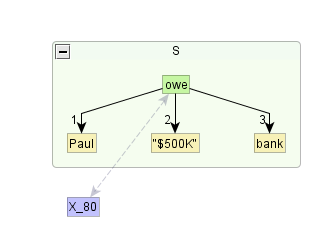
\includegraphics[width=0.6\textwidth, trim = {0cm 0cm 0cm 0cm},clip]{ch3/figs/inspecteur_root.png}
	\vspace{-0.5cm}
	\caption{application de root\_standard}
	\label{fig:rootstand}
\end{figure}

\subsubsection{lex standard : owe (satisfait les contraintes du noeud)}
Par la suite, la règle de lexicalisation standard s'applique. Cela est possible parce que le système regarde dans le semanticon pour l'unité sémantique dans le graphe d'input. Si elle existe dans le semanticon, alors il regarde ce qu'il y a à l'intérieur. Elle renferme deux lexicalisations possibles : owe et debt. Donc on va tenter ces deux lexèmes pour voir si ça fonctionne. Effectivement le système permet de prendre owe puisque owe est un verbe et qu'il satisfait la contrainte. Mais il permet aussi de prendre debt car celui-ci incorpore des verbes supports qui peuvent satisfaire la contrainte de root. Ainsi, un mécanisme complexe de lexicalisation permettra de prend un noeud sémantique en input et de le scinder en deux lors de l'arborisation. Le verbe support deviendra la racine dans ce cas. et le mot debt deviendra un de ses dépendants. Mais nous n'entreront pas dans les détails. POur cela nous vous renvoyons à Lambrey et Lareau-Lambery. Donc nous constatons qu'à ce point, plusieurs arborisation sont possibles, mais nous choisissons de travailler avec la lexicalisation simple. C'est pourquoi nous optons pour l'arborisation qui prend le verbe owe comme racine. 
\begin{figure}[htb]
	\centering
	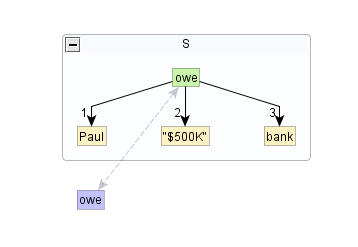
\includegraphics[width=0.7\textwidth, trim = {0cm 0cm 0cm 0cm},clip]{ch3/figs/lex_standard_root.png}
		\vspace{-0.5cm}
	\caption{application de lex\_standard}
	\label{fig:lexstand1}
\end{figure}

\subsubsection{actant gp : crée les branches et les noeuds vides}
Une fois que owe est lexicalisé, cela déclenche l'application de la règle actant\_gp. Pour chaque relation actancielle, elle puise dans le patron de régime de l'entrée lexicale quelconque. Puis elle fait la conversion des actants sémantiques en actants syntaxiques. OWe a trois actants sémantiques dans l'input. Ils seront réalisés en actants syntaxiques en fonction de la diathèse de cette entrée. (parler de la diathèse). Le patron de régime\draft{utiliser la macro pour gp} de owe impose des restrictions aux actants syntaxiques. La partie de discours doit être X. Au bout de ces branches nouvellement ajoutées, on crée des noeuds vides, mais contraints par une partie du discours spécifique.
\begin{figure}[htb]
	\centering
	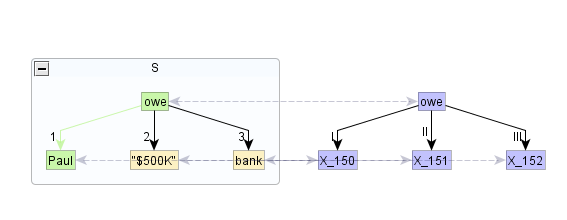
\includegraphics[width=1\textwidth, trim = {0cm 0cm 0cm 0cm},clip]{ch3/figs/actant_gp1.png}
	\caption{application de actant\_gp}
	\label{fig:actantgp}
\end{figure}

\subsubsection{lex class et lex standard}
Donc, la suite des choses est de répétée la phase de lexicalisation puisque nous avons des noeuds non-étiquetés. Alors on regarde l'unité sémantique spécifiée dans l'input qui est 'bank' 'paul' '\$500'. On va donc regarder dans le semanticon s'ils s'y trouvent. On trouvera 'bank' et sa lexicalisation 'bank' mais pas 'Paul' ni '\$500' car ceux-ci ont le trait 'class' en input. Donc lex\_standard s'applique et on lexicalise 'bank' au noeud du IIIe\draft{comment mettre le petit e} actant syntaxique car il satisfait les contraintes du noeud. Effectivement, dans le lexicon 'bank' est de type dpos=N ce qui correspond à la contrainte demandée par la règle actant\_gp précédement via le gp du verbe owe. Pour ce qui est de 'Paul' et '\$500', ils ont le trait class dans l'input sémantique. C'est là que la règle de lex\_class entre en ligne de compte. Elle passer directement au lexicon, puisque les sens ne sont pas encodés dans le semanticon comme les classes ont des comportements prédictibles. Dans le lexicon par contre, c'est là que les classes sont décrites. Effectivement la classe proper\_noun et la classe numeral vont permettre l'application de la règle lex\_class et de lexicaliser paul et 500 piastres. Les classes ont les informations de type dpos et autres traits grammaticaux. L'étiquette du noeud sémantique est directement copiée en syntaxe. on s'assure finalement que les contraintes de ces classes respectent les contraintes du noeuds généré par gp\_actant. Lorsque c'est le cas, la lexicalisation se produit. Les noms propres héritent des traits de la classe des noms, donc la dpos est là, puis les montants héritent des traits de la classe des nombres.

\begin{figure}[htb]
	\centering
	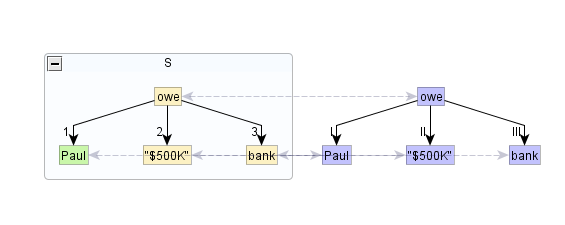
\includegraphics[width=1\textwidth, trim = {0cm 0cm 0cm 0cm},clip]{ch3/figs/lex_standard2.png}
	\caption{application de lex\_standard}
	\label{fig:lexstand2}
\end{figure}

\subsubsection{traits grammaticaux}
\draft{transfert des traits: définitude, temps, aspect, nombre,etc. }


\subsection{2ème phase: RSyntP à RSyntS}

\subsubsection{lex class et lex lu}
On va chercher les lexicalisations de surface de chacune des unités lexicales. Provenant des classes et des entrées directement. \draft{demander à françois à quoi sert cette étape}. Lex class fait paul et 500 , puis lex lu fait bank et owe.
\begin{figure}[htb]
	\centering
	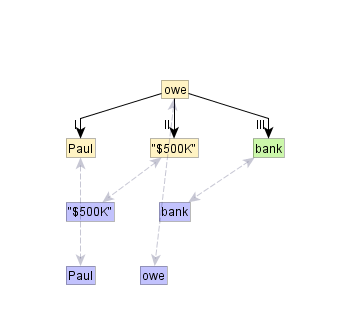
\includegraphics[width=0.7\textwidth, trim = {0cm 0cm 0cm 0cm},clip]{ch3/figs/rsyntslexicalisation1.png}
	\caption{application de lex class et lex lu}
	\label{fig:lexsurf}
\end{figure}

\subsubsection{synt actant subj}
Réalise la relation subjectale entre le verbe et le nom qui a cette relation. Cette information est encodée dans le gp du verbe owe qui est hérité de verb dit, puis de verb dt jusqu'à verb tout court. Qui dit que son premier actant I, est le sujet. \lstinline!gp = { I = { dpos = N rel = subjective } } !

\subsubsection{synt actant dir}
Crée la relation d'objet direct entre le verbe et l'actant II. Cela est encodé via le verbe owe, qui est un verbe dit, donc hérité de verb dt, qui a comme info que son IIe actant correspond à la relation objet direct.  \lstinline!gp = { II = { dpos = N  rel = dir_objective } }!

\subsubsection{synt actant prep}
Celle-ci est la plus complexe des règles actancielles de surface. Car elle va prendre un noeud syntaxique profond et le scinder en 2 pour réaliser le mot fonctionnel qu'est la préposition.  \lstinline! gp = {III = {  dpos = N  rel = indir_objective  prep = to  }  }!

\subsubsection{det def}

Cette règle de surface ajoute les déterminants.Elle est la seule qui est propre à l'anglais parmi les règles présentées puisque \lex{the} est uniquement un déterminant en anglais.

La figure \ref{fig:syntsurf} démontre l'application simultanée de toutes ces règles de surface.

\begin{figure}[htb]
	\centering
	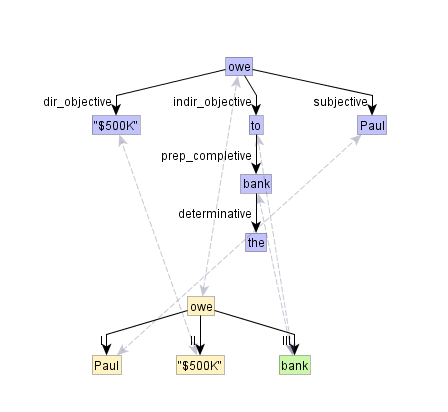
\includegraphics[width=0.7\textwidth, trim = {0cm 0cm 0cm 0cm},clip]{ch3/figs/rsynts_syntactisation.png}
	\caption{application de subj,dir,prep et det}
	\label{fig:syntsurf}
\end{figure}

%%%%%%%%%%%%%%%%%%%%%%%%%%%%%%%%%%%%%%%%%%%%%%%%
% --------- P R O B L É M A T I Q U E ---------
%%%%%%%%%%%%%%%%%%%%%%%%%%%%%%%%%%%%%%%%%%%%%%%%

\section{Problématique}\label{problema}

Le système que nous venons de présenter performe très bien d'un point de vue des phénomènes langagiers complexes et profonds. Toutefois, le dictionnaire lexical de GenDR ne couvre que les 1500 lexies les plus fréquentes du langage. Ainsi, pour accéder à une plus grande couverture du langage, GenDR nécessite principalement l'accès aux informations lexicales encodées dans les verbes. Car, puisque les verbes sont au centre des énoncés (ce qui est expliqué par la règle d'arborisation de création de la racine propre à MARQUIS, FORGe et GenDR), on devrait avoir leurs informations lexicales dans nos dictionnaires, ils sont vitaux. Comme le dit \cite{SchulerVerbnetBroadcoverageComprehensive2005}:
\begin{quotation} In particular, since verbs often convey the main idea of a sentence, such a resource must represent verb meanings. These require a particularly precise and well deffined representation that captures both their predicate-argument structure as well as their semantic content.\end{quotation}

La raison d'être de ce mémoire prend place dans ce contexte. Comme VerbNet, korhonen et Messiant le dit, pour que des applications soient capables de représenter les langues naturelles, elles nécessitent des ressources pouvant l'aider à couvrir large. Avec un dictionnaire de patron de régime, GenDR pourrait couvrir la plupart des énoncés du parler quotidien de la langue anglaise. Il n'y aurait même pas besoin de se doter des patrons de régime des autres discours puisque les comportements syntaxiques des autres parties du discours sont beaucoup plus prévisibles. Nom (comp du nom) Adv (modificateur) Adj (modificateur). Il bénéficeerait très clairement des régimes ceux-ci, mais les verbes permettraient une couverture bcp plus importante d'un coup. C'est pourquoi nous avons décidé d'implémenter un dictionnaire verbal de patron de régime à ce réalisateur profond. Avant d'aller plus loin, nous devons élucider ce que sont les patrons de régime.

\section{Patrons de régime}

Les patrons de régime décrivent les cooccurrences syntaxiques des unités lexicales \citep{MilicevicSchemaregimepont2009}. La cooccurrence de la lexie avec ses actants. Autrement dit les sujets et objets des verbes, les compléments du nom. Ceux-ci correspondent aux actants syntaxiques de surface. Le patron de régime encode des relations plus profondes comme les actants syntaxiques profonds. Les patrons de régime d'une lexie correspondent à l'ensemble des constructions syntaxiques dont la lexie est la gouverneure. Les actants syntaxiques en sont ses dépendants. On les encode dans un dictionnaire car les patrons de régime des lexies ne sont généralement pas prévisibles. Effectivement, on ne peut pas prédire les patrons de régime des unités lexicales d'une langue. D'ailleurs, même des verbes sémantiquement proches ne possèderont pas nécessairement les mêmes constructions syntaxiques ex de Milicevic p. 95( se souvenir de X , mais se rappeler X ). Le nombre d'actant n'est pas prévisible non plus en regardant l'unité lexicale à partir de son sens. 

Puisque les arguments sélectionnés par une lexie sont généralement idiosyncratiques, on encode ces comportements syntaxiques dans des dictionnaires.

les GP encodent la diathèse (correspondance entre les actants sémantiques d'une lexie et ses actants syntaxiques profonds) et la réalisation des actants (I à sujet II objet direct, indirect, ou oblique). La diathèse peut soit être triviale (1 pour I, 2 pour II, etc.) ou pas (1 -II et 2-I)

Le patron de régime d'une lexie encode les correspondances entre ses actants (au niveau sémantique, syntaxique profond et syntaxique de surface), les moyens morpho-syntaxiques d'expressions des actants et les restriction sur les actants.

Plus tôt dans le chapitre nous avions parlé de l'interface sémantique-syntaxe et de l'importance des règles sémantiques qui font la transition entre Rsem et RSyntP. Le rôle le plus important du GP est de fournir l'information nécessaire au passage de la sem à la synt lors des opérations de lexicalisation et d’arborisation. 

\begin{quotation}{Comme le choix lexical détermine le choix des constructions syntaxiques possibles (la lexie sélectionnée « amène » avec elle son régime) et vice-versa (le choix d’une structure impose certains choix lexicaux), on peut dire que c’est le schéma de régime qui, au sein d’un MST, fait le pont entre le lexique et la grammaire. \citep{MilicevicSchemaregimepont2009}, p.105}
\end{quotation}

GenDR bénéficierait énormément d'un dictionnaire de patron de régime. Notamment parce que le logiciel MATE présente des limites d'encodage quant à la manière dont les gp sont encodés présentement dans GenDR. Pour un verbe donné, on ne peut pas avoir deux parties du discours différentes qui compétitionnent pour la même position syntaxique. Autrement dit, prenons le cas de X (exemple). Cela restreint le nombre de génération possible pour un verbe ou bien ça peuple inutilement le dictionnaire d'entrée verbale par partie du discours qu'il prend. Ce n'est pas une manière efficace d'encoder le langage. C'est là qu'un dictionnaire de patron de régime entre en ligne de compte. Et ça permet une grande couverture de la langue. Sans dictionnaire de patron de régime ni d'acquisition automatique de ceux-ci, il faut les encoder à la main un par un. Ce n'est pas une tâche rationnelle.

Nous nous sommes finalement retourner vers VerbNet. Le chapitre suivant décrit cette ressource lexicale et les autres que nous avons évaluées.